\documentclass[12pt]{article}
\pagenumbering{gobble}
\usepackage[margin=1in]{geometry}
\title{\textit{Tricky Logic Puzzles for Adults}\\
Calcudoku Puzzle Teaser}
\author{Steven Clontz | clontz.org}
\usepackage{tikz}
\date{}
\begin{document}
\fontfamily{cmss}\selectfont
\maketitle
\begin{center}\small
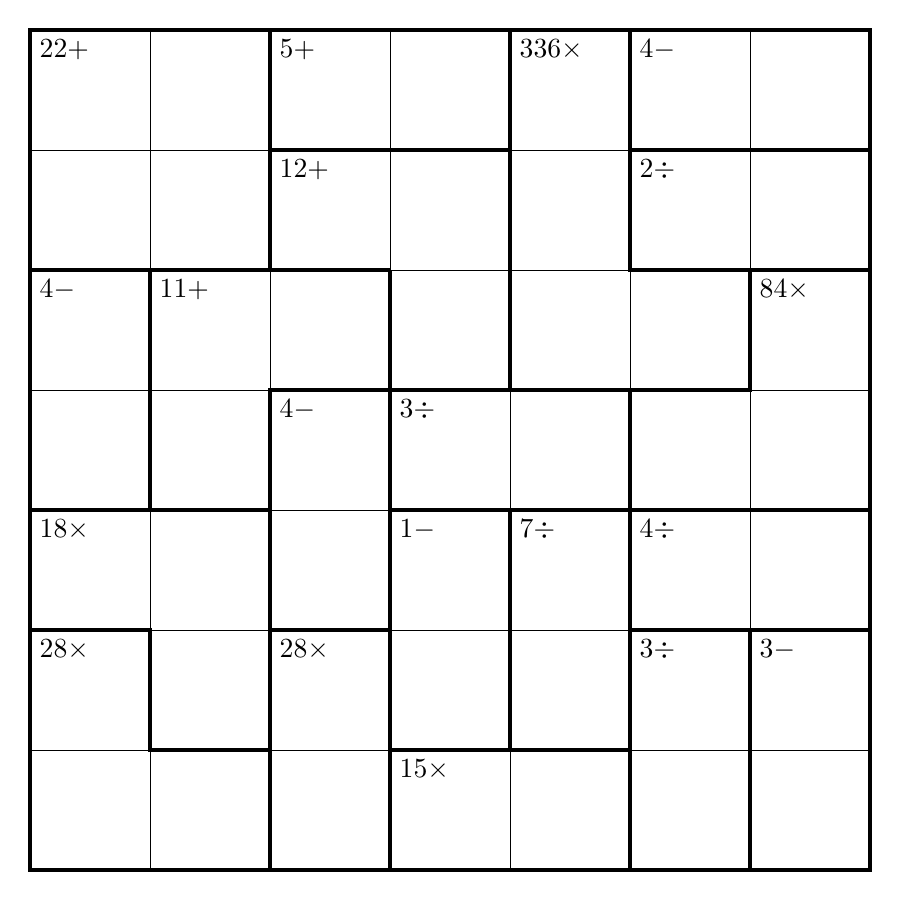
\begin{tikzpicture}[x=0.6in,y=0.6in]
\draw[very thin,step=1] (0,0) grid (7,7);
\draw[ultra thick] (0,5) rectangle (2,7);
\draw[ultra thick] (2,6) rectangle (4,7);
\draw[ultra thick] (2,5) -- (3,5);
\draw[ultra thick] (5,7) -- (4,7) -- (4,4) -- (6,4) -- (6,5);
\draw[ultra thick] (5,6) rectangle (7,7);
\draw[ultra thick] (5,5) rectangle (7,6);
\draw[ultra thick] (0,3) rectangle (1,5);
\draw[ultra thick] (1,3) -- (2,3) -- (2,4) -- (3,4) -- (3,5);
\draw[ultra thick] (2,2) rectangle (3,4);
\draw[ultra thick] (3,3) rectangle (5,4);
\draw[ultra thick] (5,3) -- (7,3) -- (7,5);
\draw[ultra thick] (0,3) -- (0,2) -- (1,2) -- (1,1) -- (2,1) -- (2,3);
\draw[ultra thick] (0,2) -- (0,0) -- (2,0) -- (2,1);
\draw[ultra thick] (2,0) rectangle (3,2);
\draw[ultra thick] (3,1) rectangle (4,3);
\draw[ultra thick] (3,0) rectangle (5,1);
\draw[ultra thick] (4,1) rectangle (5,3);
\draw[ultra thick] (5,2) rectangle (7,3);
\draw[ultra thick] (5,0) rectangle (6,2);
\draw[ultra thick] (6,0) rectangle (7,2);
\node[anchor=north west] at (0,7) {\(22+\)};
\node[anchor=north west] at (2,7) {\(5+\)};
\node[anchor=north west] at (4,7) {\(336\times\)};
\node[anchor=north west] at (5,7) {\(4-\)};
\node[anchor=north west] at (2,6) {\(12+\)};
\node[anchor=north west] at (5,6) {\(2\div\)};
\node[anchor=north west] at (0,5) {\(4-\)};
\node[anchor=north west] at (1,5) {\(11+\)};
\node[anchor=north west] at (6,5) {\(84\times\)};
\node[anchor=north west] at (2,4) {\(4-\)};
\node[anchor=north west] at (3,4) {\(3\div\)};
\node[anchor=north west] at (0,3) {\(18\times\)};
\node[anchor=north west] at (3,3) {\(1-\)};
\node[anchor=north west] at (4,3) {\(7\div\)};
\node[anchor=north west] at (5,3) {\(4\div\)};
\node[anchor=north west] at (0,2) {\(28\times\)};
\node[anchor=north west] at (2,2) {\(28\times\)};
\node[anchor=north west] at (5,2) {\(3\div\)};
\node[anchor=north west] at (6,2) {\(3-\)};
\node[anchor=north west] at (3,1) {\(15\times\)};
\end{tikzpicture}
\end{center}
\end{document}
